% ============================================
%       Presentation Compile Setting
% ============================================

\documentclass[8pt, aspectratio=169]{beamer} % for full presentation
% \documentclass[8pt, aspectratio=169, handout]{beamer} % without animation and notes
% \documentclass[8pt, aspectratio=169, handout, draft]{beamer} % for draft mode
% \documentclass[8pt, aspectratio=169, handout]{beamer} \setbeameroption{show only notes} % for notes only

% ============================================
%           MIC Lab template
% ============================================
\newcommand{\template}{../template}

% \input{\template/macros/macros_general.tex}
% \input{\template/macros/macros_math.tex}
% \input{\template/symbols/symbols_NN.tex}
% \input{\template/symbols/symbols_robot.tex}
% Add more macros/symbols as needed

\newcommand{\logoOne}{\template/figs/logo_KAIST_simple.png}
\newcommand{\logoTwo}{\template/figs/logo_MIC.png}
\newcommand{\logoTopRight}{\template/figs/logo_MIC_white.png}

% ============================================
%           Flux Theme
% ============================================

% Use roboto Font (recommended)
% \usepackage[sfdefault]{roboto}
\usepackage[utf8]{inputenc}
\usepackage[T1]{fontenc}

% Define where theme files are located. ('/styles')
\usepackage{styles/fluxmacros}
\usefolder{styles}
% Use Flux theme v0.1 beta
% Available style: asphalt, blue, red, green, gray, dding (custom)
\usetheme[style=dding]{flux}

% ============================================
%         Additional Packages
% ============================================

\usepackage{booktabs}
\usepackage{colortbl}
\usepackage{ragged2e}
\usepackage{schemabloc}
\usepackage{multirow}
\usepackage{multicol}
\usepackage{kotex}
\usepackage{media9}
\usepackage{pgfpages}
% \setbeameroption{show notes} % Show notes separately
% \setbeameroption{show notes on second screen=right} % Show notes on the presenter screen

% ============================================
%         Colors and Macros
% ============================================

% https://latexcolor.com % color list
\definecolor{airforceblue}{rgb}{0.36, 0.54, 0.66}
\definecolor{awesome}{rgb}{1.0, 0.13, 0.32}
\newcommand{\ctxt}[2]{{\color{#1}{#2}\color{black}}}
\newcommand{\cred}[1]{{\ctxt{awesome}{#1}}}
\newcommand{\cblue}[1]{{\ctxt{airforceblue}{#1}}}

% ============================================
%         Title Page
% ============================================
\title{
    Safe Reinforcement Learning
} 
\subtitle{
    % \textit{Where}\\
}
\author{
  \textbf{\cblue{Minseok Seo}}\inst{1},  % Emphasize the presenter!
}
\date{{September 5, 2025}}
\institute{%
    \begin{minipage}[c]{\linewidth}
      \centering
      \inst{1}%
      Mobility Intelligence and Control Laboratory (MIC Lab) \\
      CCS Graduate School of Mobility \\
      Korea Advanced Institute of Science and Technology (KAIST)
  \end{minipage}
}
\setbeamerfont{institute}{size=\normalsize}

\titlegraphic{\logoTopRight}

%~~~~~~~~~~~~~~~~~~~~~~~~~~~~~~~~~~~~~~~~~~~~~~~~~~~~~~~~~~~~~~~~~~~~~~~~~~~~~~
\AtBeginSection[]{%
  \frame<beamer>{ 
    \frametitle{Outline}   
    \tableofcontents[currentsection] 
  }
}

% Use the following code to show section and subsection titles at the beginning of each section and subsection
% \AtBeginSubsection[]{%
%   \begin{frame}
%   \vfill
%   \centering
%     \insertsectionhead
%     \\
%     \large\textbf{\insertsubsectionhead}
%   \vfill
%   \end{frame}
% }
%~~~~~~~~~~~~~~~~~~~~~~~~~~~~~~~~~~~~~~~~~~~~~~~~~~~~~~~~~~~~~~~~~~~~~~~~~~~~~~

\begin{document}

%~~~~~~~~~~~~~~~~~~~~~~~~~~~~~~~~~~~~~~~~~~~~~~~~~~~~~~~~~~~~~~~~~~~~~~~~~~~~~~
\titlepage 

\begin{frame}{Outline}
  \tableofcontents
\end{frame}
%~~~~~~~~~~~~~~~~~~~~~~~~~~~~~~~~~~~~~~~~~~~~~~~~~~~~~~~~~~~~~~~~~~~~~~~~~~~~~~

% ============================================
%         Introduction
% ============================================

\section{Introduction}

%~~~~~~~~~~~~~~~~~~~~~~~~~~~~~~~~~~~~~~~~~~~~~~~~~~~~~~~~~~~~~~~~~~~~~~~~~~~~~~

\subsection{Motivation}

\begin{frame}{\insertsubsectionhead}{Autonomous Driving}


  \vspace{0.5cm}

  {
    \begin{figure}
      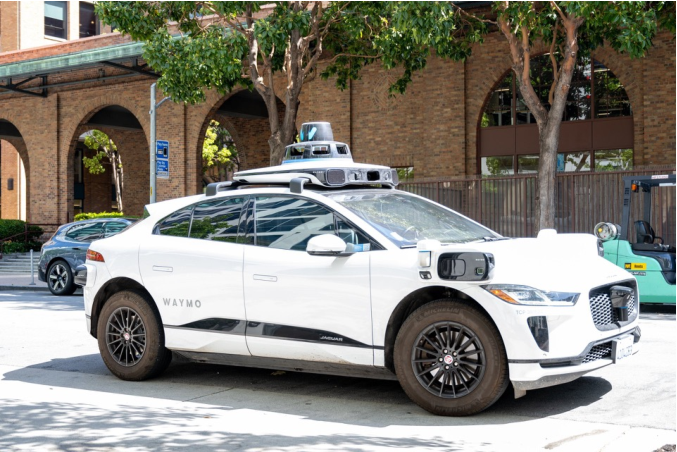
\includegraphics[width=0.45\textwidth]{figures/waymo.pdf}
      \hspace{1cm}
      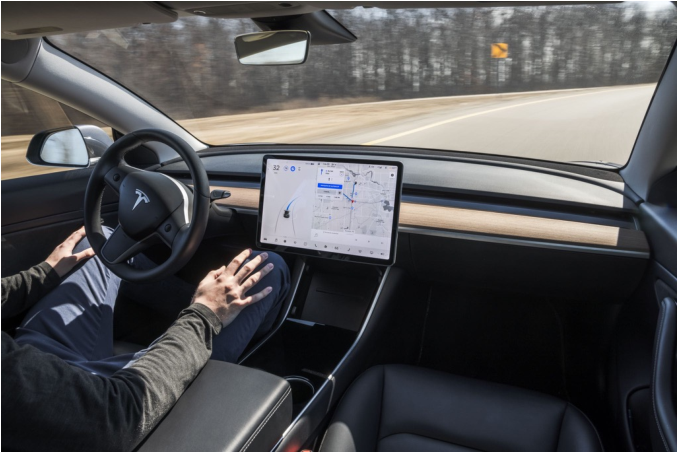
\includegraphics[width=0.45\textwidth]{figures/tesla.pdf}
      \caption{Waymo and Tesla}
    \end{figure}
  }

\end{frame}

\note[enumerate]
{
  \item You can add notes like this.
  \item These notes will not be shown in the presentation.
}

\begin{frame}{\insertsubsectionhead}{Supervised Learning}

  \vspace{0.5cm}

  {
    \begin{figure}
      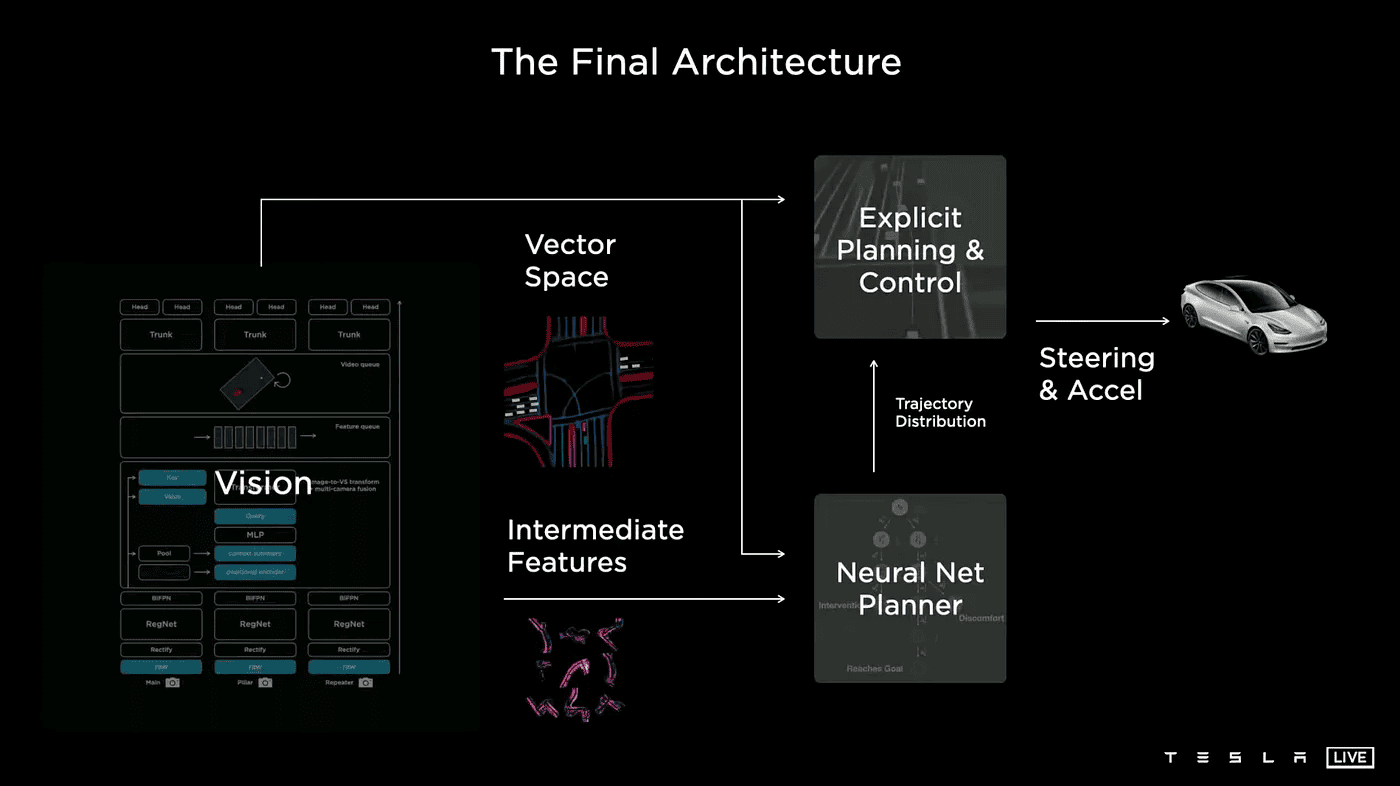
\includegraphics[width=0.7\textwidth]{figures/tesla-architecture.png}
      \caption{Tesla's Architecture in 2021 (source: \href{https://www.youtube.com/live/j0z4FweCy4M?si=vEB4egdqDOVpmpLu}{AI Day 2021})}
    \end{figure}
  }
\end{frame}

\begin{frame}{\insertsubsectionhead}{Supervised Learning}

  {
    \begin{figure}
      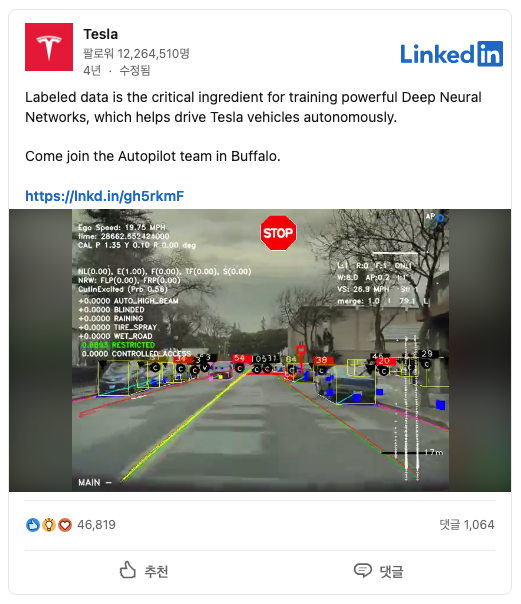
\includegraphics[width=0.25\textwidth]{figures/tesla-label.png}
      \caption{Tesla’s recruitment post for data labeling positions}
    \end{figure}

    \onslide <1->
    {
      \begin{itemize}
        \item <2-> Supervised learning requires \textcolor{red}{a large amount of labeled data.}
        \item <3-> Since it is created by humans, it is \textcolor{red}{expensive.}
        \item <4-> The performance of supervised learning is \textcolor{red}{limited by human-labeled data.}
      \end{itemize}
    }
  }

\end{frame}

%~~~~~~~~~~~~~~~~~~~~~~~~~~~~~~~~~~~~~~~~~~~~~~~~~~~~~~~~~~~~~~~~~~~~~~~~~~~~~~

\subsection{Reinforcement Learning (RL)}

\begin{frame}{\insertsubsectionhead}

  \centering
  \begin{columns}[T,totalwidth=\textwidth]
    % Alphago
    \column{0.32\textwidth}
      \centering
      \textbf{Alpha Go} \cite{silver2016mastering}
      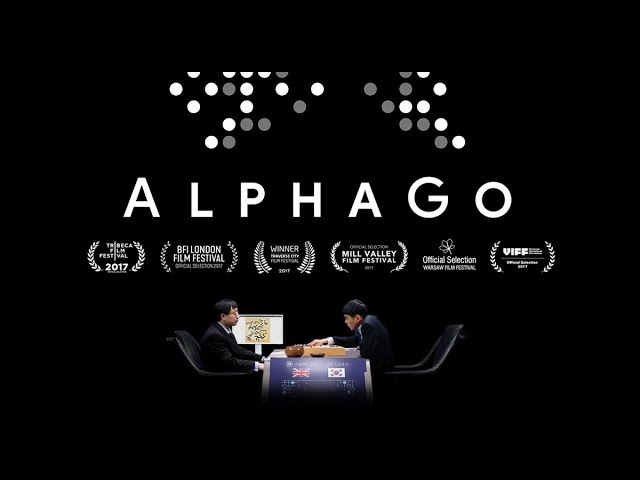
\includegraphics[width=\linewidth,height=0.5625\linewidth]{figures/alphago.jpg}

    % DQN
    \column{0.32\textwidth}
      \centering
      \textbf{Deep Q-Network} \cite{mnih2013playing}
      \includemedia[
        width=\linewidth,
        height=0.5625\linewidth,
        activate=pageopen,
        addresource=figures/dqn.mp4,
        flashvars={source=figures/dqn.mp4&autoPlay=true&loop=true}
      ]{}{VPlayer.swf}

    % Walker
    \column{0.32\textwidth}
      \centering
      \textbf{Proximal Policy Optimization} \cite{schulman2017proximal}
      \includemedia[
        width=\linewidth,
        height=0.5625\linewidth,
        activate=pageopen,
        addresource=figures/walker.mp4,
        flashvars={source=figures/walker.mp4&autoPlay=true&loop=true}
      ]{}{VPlayer.swf}
  \end{columns}

\end{frame}

\begin{frame}{\insertsubsectionhead}

  \begin{figure}
    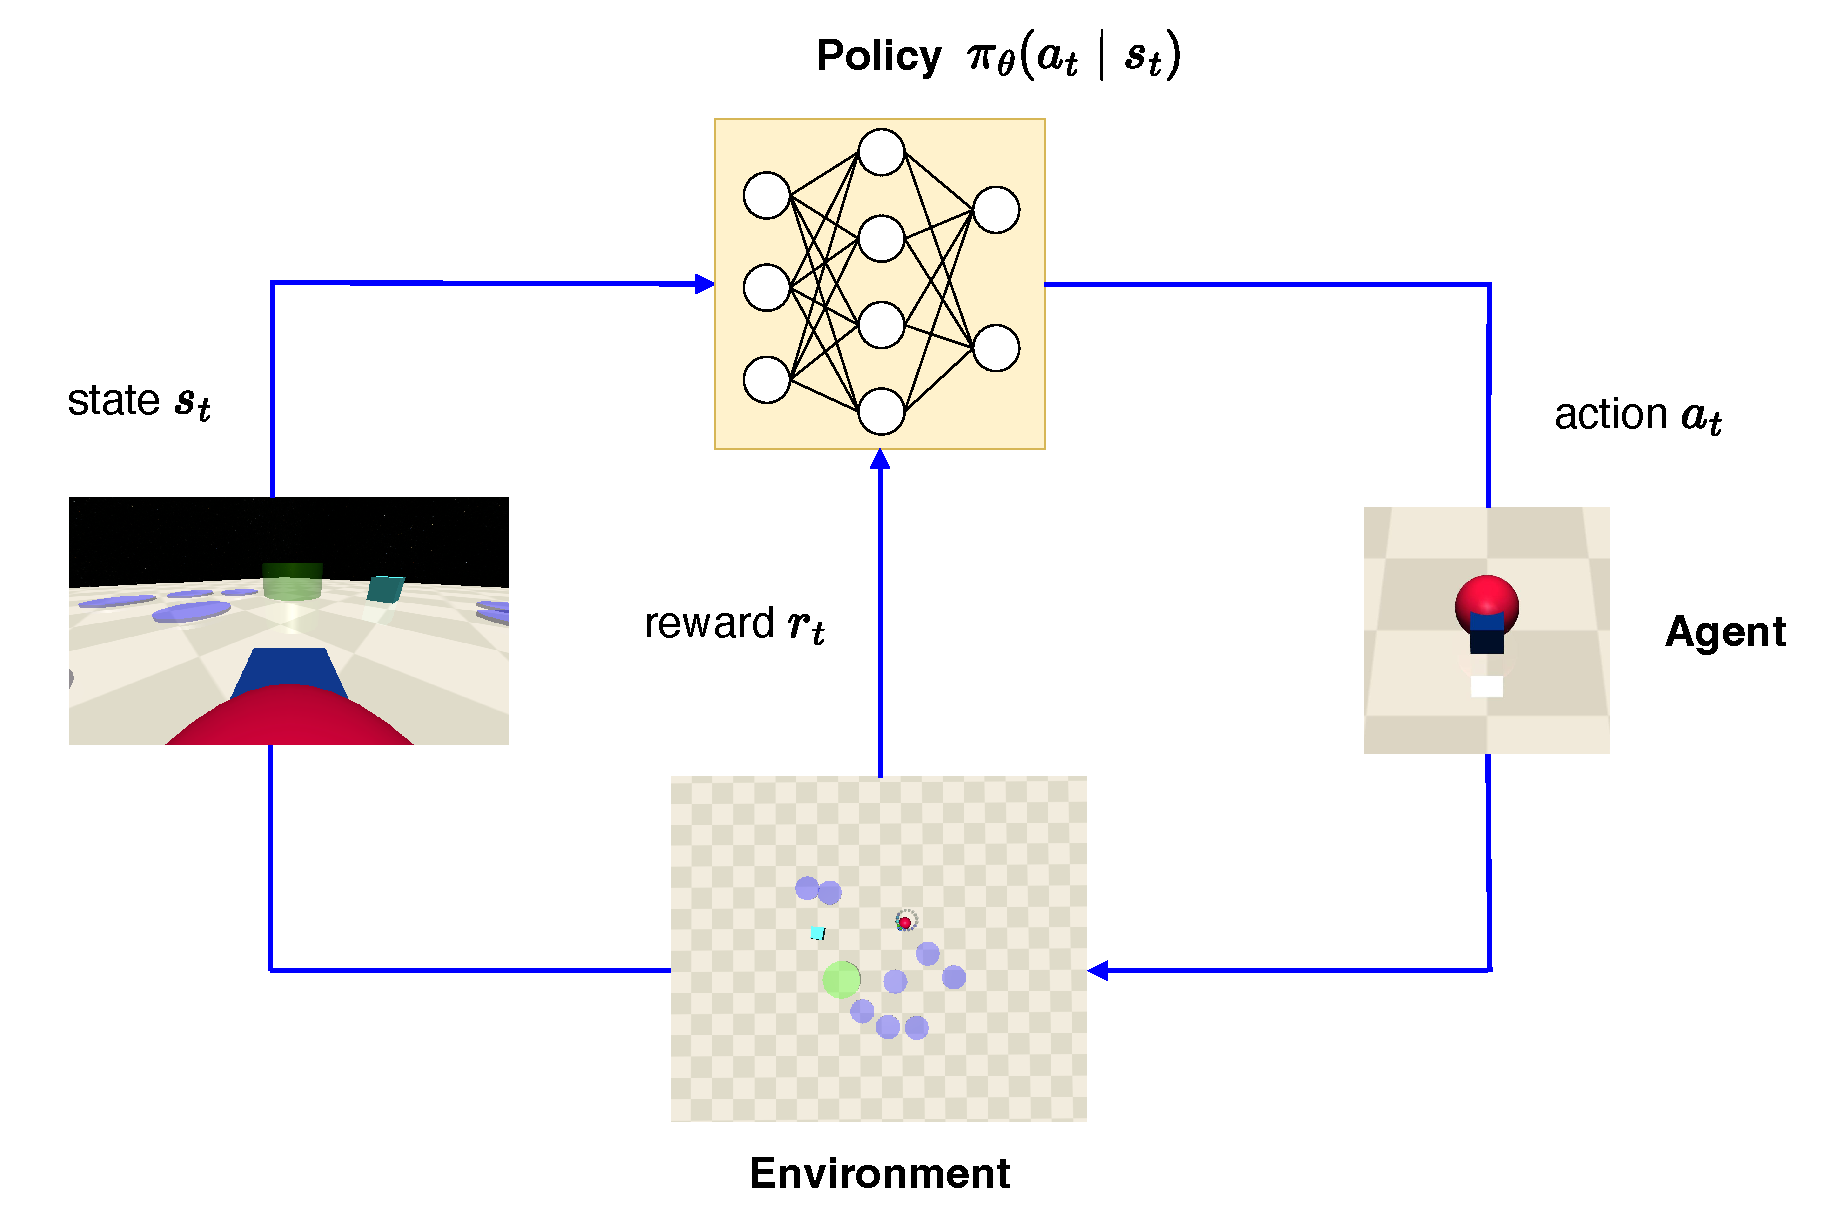
\includegraphics[width=0.6\textwidth]{figures/rl1.pdf}
    \caption{Overview of the reinforcement learning framework}
  \end{figure}

\end{frame}

\begin{frame}{\insertsubsectionhead}

  \begin{figure}
    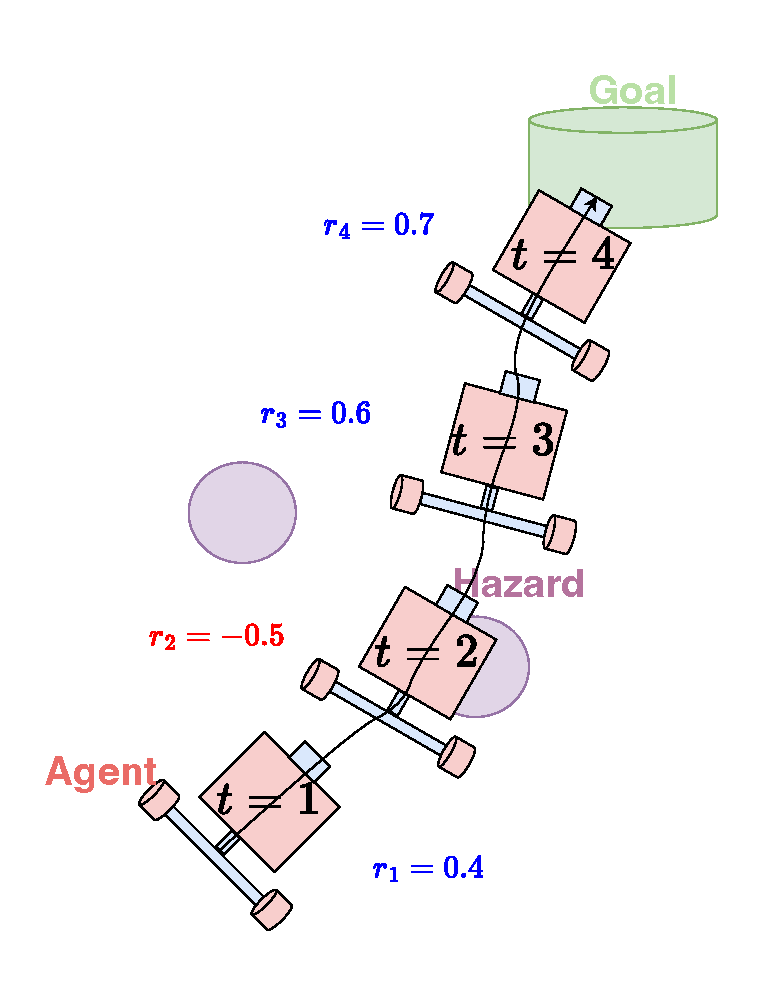
\includegraphics[width=0.3\textwidth]{figures/rl2.pdf}
    \caption{Illustration of sequential decision making: the agent receives a reward after each action.}
  \end{figure}

\end{frame}


\begin{frame}{\insertsubsectionhead}

  \begin{figure}
    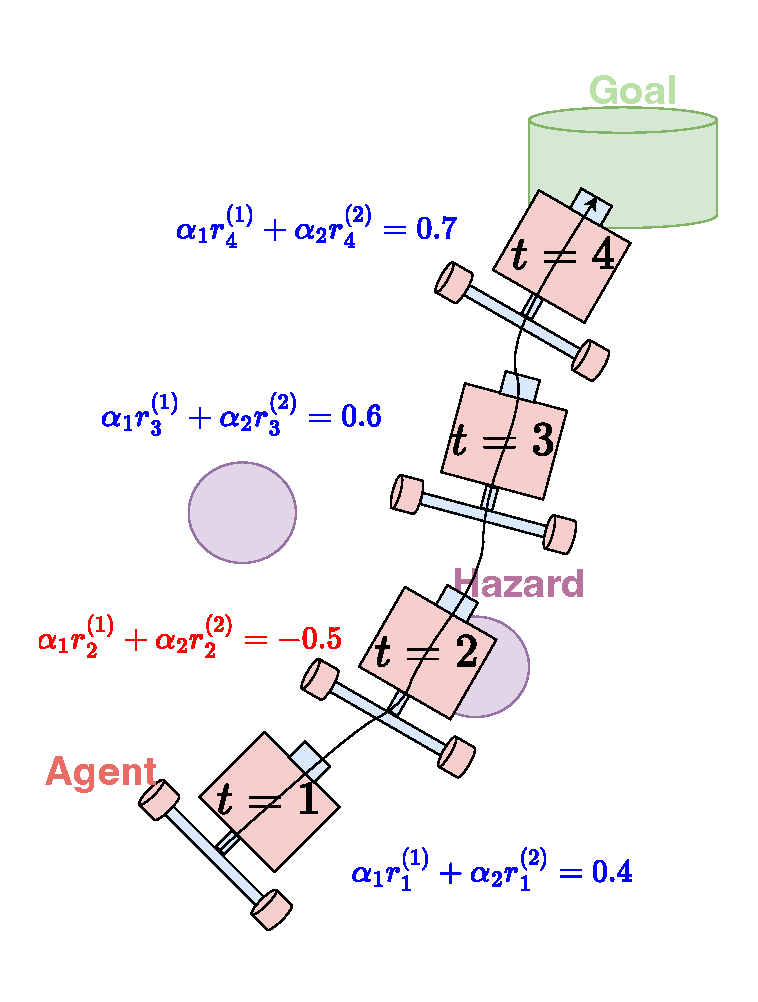
\includegraphics[width=0.3\textwidth]{figures/reward-engineering.pdf}
    \caption{Illustration of reward engineering: shaping the reward signal to guide the agent's learning process.}
  \end{figure}

\end{frame}

\begin{frame}{\insertsubsectionhead}{Objective of RL}
  \begin{itemize}
    \item Policy parameterized by $\theta$, denoted as $\pi_\theta(a|s)$
    \item Goal: find the optimal policy $\pi^*_\theta$ that maximizes the expected cumulative reward
  \end{itemize}

  \begin{equation}
    \begin{aligned}
      \theta^* &= \arg\max_\theta J(\theta) \\
      J(\theta) &= \mathbb{E}_{\tau \sim \pi_\theta} \left[\sum^T_{t = 0} r_t \right]
    \end{aligned}
  \end{equation}

\end{frame}


\begin{frame}{\insertsubsectionhead}{Challenges of RL}

  \begin{enumerate}
    \item<1-> Needs \textcolor{red}{simulation}, not labeled data
    \item<2-> Works in simulation, but may fail in the real world
      \begin{itemize}
        \item<2-> Even after training, the agent may still take \textcolor{red}{unsafe actions}
      \end{itemize}
    \item<3-> \textcolor{red}{Reward engineering} can induce desired behaviors (multi-objective), but it is time-consuming and difficult
  \end{enumerate}

  \uncover<4->{
    \begin{block}{My research}
      Challenges 2 \& 3: learning safe policies without relying on reward engineering
    \end{block}
  }
\end{frame}

% \begin{frame}{\insertsubsectionhead}

%   \begin{enumerate}
%     \item <1-> RL does not require labeled data; instead, \textcolor{red}{it needs simulation.}
%     \item <2-> Even if works well in simulation, \textcolor{red}{it may not performs as expected in the real world.}
%     \item <3-> Through reward engineering, desired behaviors (multi-objective) can be induced, but \textcolor{red}{this is a very time-consuming and difficult task.}
%   \end{enumerate}

%   \uncover<4->{
%     \begin{block}{My research}
%       Challenge 3: learning policies that achieve objectives while satisfying constraints, without relying on reward engineering.
%     \end{block}
%   }

% \end{frame}

% ============================================
%         Constrained RL Page
% ============================================

\section{Constrained Reinforcement Learning}

%~~~~~~~~~~~~~~~~~~~~~~~~~~~~~~~~~~~~~~~~~~~~~~~~~~~~~~~~~~~~~~~~~~~~~~~~~~~~~~

\subsection{Constrained Reinforcement Learning (Constrained RL)}

\begin{frame}{\insertsubsectionhead}
  \begin{figure}
    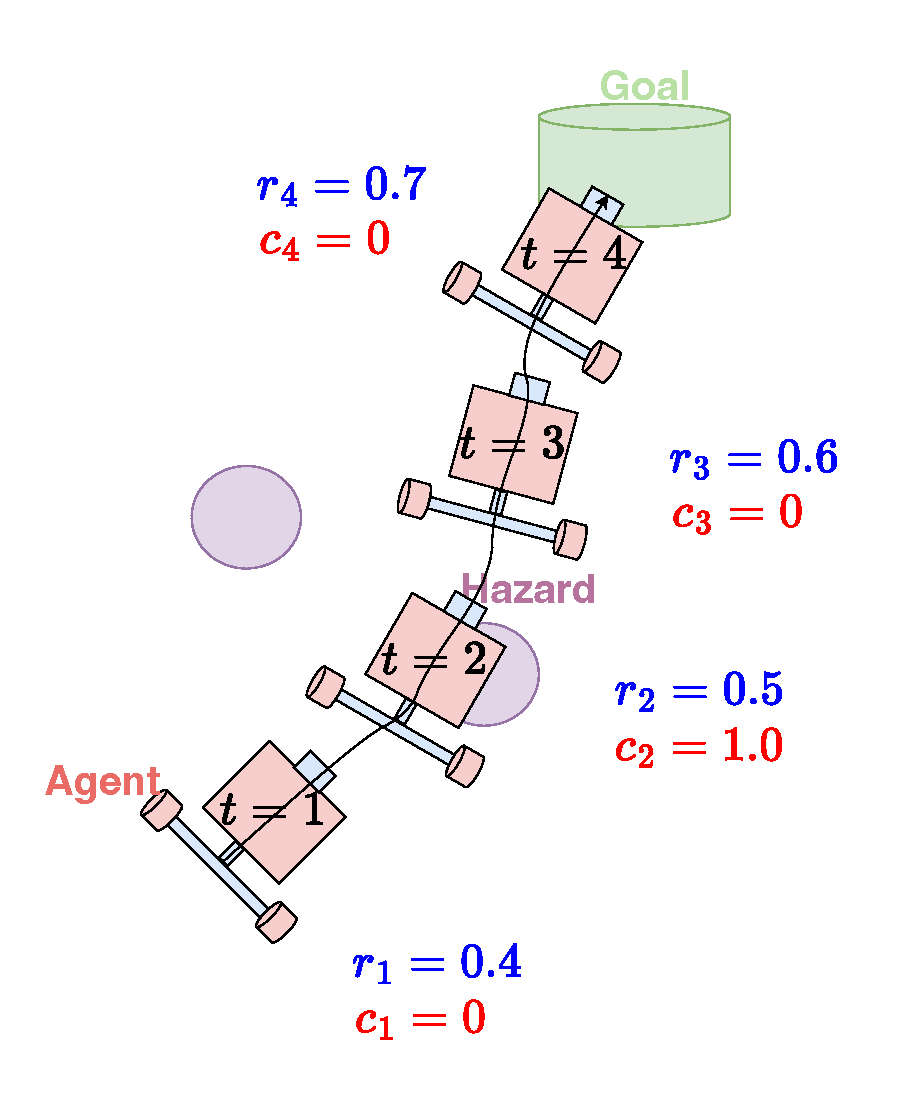
\includegraphics[width=0.35\textwidth]{figures/constrained-rl1.pdf}
    \caption{Constrained RL example — agent trajectory with rewards (blue) and costs (red)}
  \end{figure}
\end{frame}

%~~~~~~~~~~~~~~~~~~~~~~~~~~~~~~~~~~~~~~~~~~~~~~~~~~~~~~~~~~~~~~~~~~~~~~~~~~~~~~

\subsection{Constrained Policy Optimization Problem}

\begin{frame}{\insertsubsectionhead}

  \begin{equation}
    \begin{aligned}
      \theta^* &= \arg\max_\theta J(\theta) \\
      J(\theta) &= \mathbb{E}_{\tau \sim \pi_\theta} \left[ \sum^T_{t = 0} r_t \right] \; \text{subject to} \; \mathbb{E}_{\tau \sim \pi_\theta} \left[ \sum^T_{t = 0} c_t \right] \leq d
    \end{aligned}
  \end{equation}

  \vspace{0.5cm}

  \begin{itemize}
    \item <2-> Find a policy that maximizes rewards while satisfying constraints.
    \item <3-> \textcolor{red}{Directly solving constrained optimization} is difficult.
    \item <4-> By applying Lagrangian relaxation, we can \textcolor{blue}{convert it to an unconstrained problem.}
  \end{itemize}

\end{frame}

\begin{frame}{\insertsubsectionhead}

  \begin{equation}
    \begin{aligned}
      \theta^* &= \arg\max_\theta \mathcal{L}(\theta, \lambda) \\
      \mathcal{L}(\theta, \lambda) &= \mathbb{E}_{\tau \sim \pi_\theta} \left[ \sum^T_{t = 0} r_t \right] - \lambda \left( \mathbb{E}_{\tau \sim \pi_\theta} \left[ \sum^T_{t = 0} c_t \right] - d \right)
    \end{aligned}
  \end{equation}

  \vspace{0.5cm}

  \begin{equation}
    \lambda \leftarrow \left[ \lambda + \beta\left( \hat{J}_c - d \right) \right]_+
  \end{equation}

  \vspace{0.5cm}

  Penalty ($\lambda$) increases when constraints are violated → policy is encouraged to satisfy them.

  % Whenever the agent violates the constraints, the penalty (Lagrange multiplier, $\lambda$) is increased, thereby encouraging the policy to satisfy the constraints.

\end{frame}

\begin{frame}{\insertsubsectionhead}

  In CMDPs \cite{altman2021constrained}, constraints are imposed on the trajectory level.

  \begin{figure}
    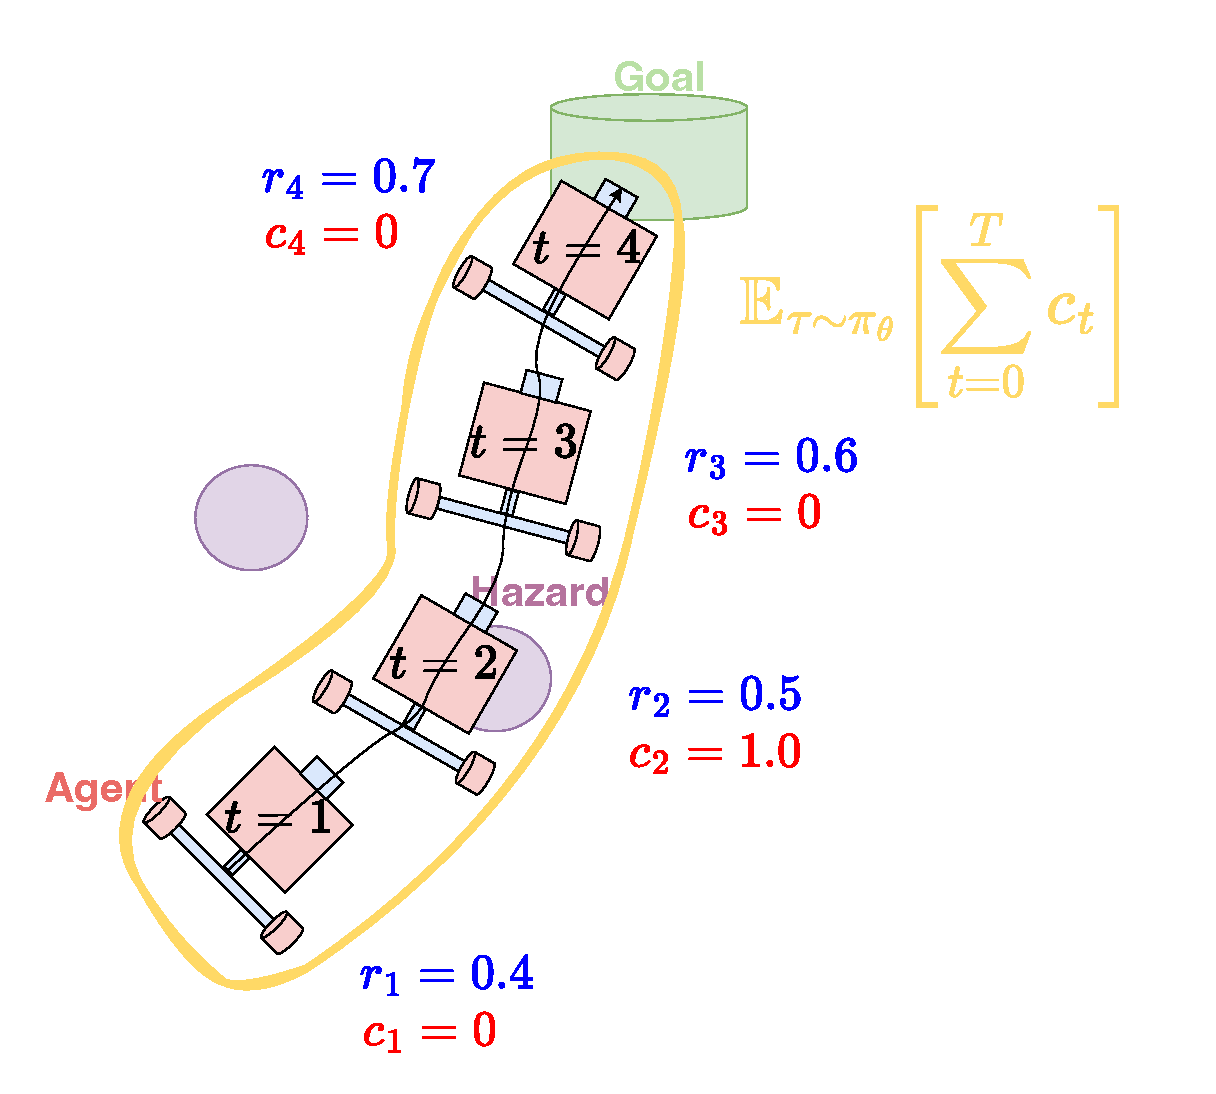
\includegraphics[width=0.3\textwidth]{figures/constrained-rl2.pdf}
    \caption{CMDP example — agent trajectory with rewards (blue) and costs (red)}
  \end{figure}

  \uncover<2->{\textbf{Wouldn’t imposing constraints at the state level allow for more precise constraint enforcement?}}

\end{frame}

%~~~~~~~~~~~~~~~~~~~~~~~~~~~~~~~~~~~~~~~~~~~~~~~~~~~~~~~~~~~~~~~~~~~~~~~~~~~~~~

\subsection{State-wise Constrained Policy Optimization}

\begin{frame}{\insertsubsectionhead}

  In state-wise constrained MDPs, constraints are imposed on each state.

  \begin{figure}
    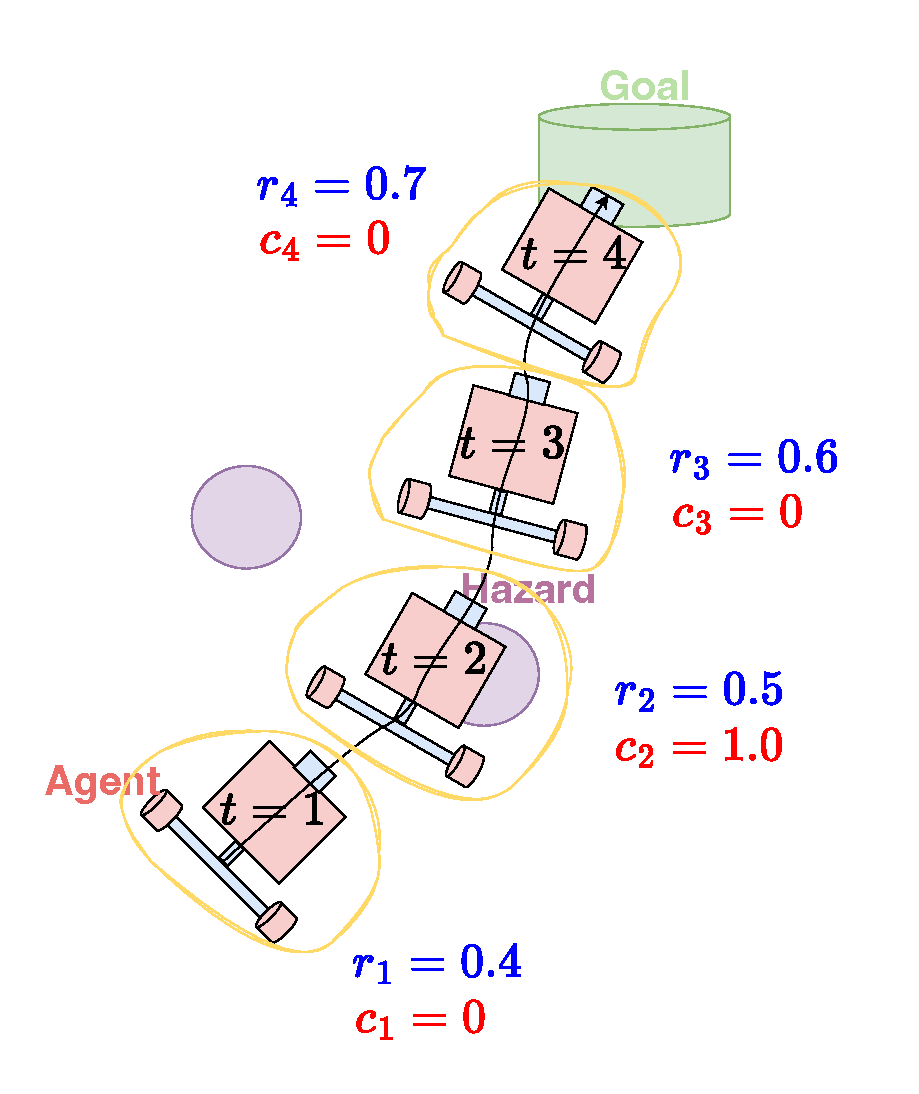
\includegraphics[width=0.25\textwidth]{figures/statewise-constrained-rl.pdf}
    \caption{State-wise constrained MDP example — agent trajectory with rewards (blue) and costs (red)}
  \end{figure}

\end{frame}

\begin{frame}{\insertsubsectionhead}{Proposed Method}

  \begin{equation}
    \begin{aligned}
      \pi^* &= \arg\max_{\pi_\theta} J(\theta) \\
      J(\theta) &= \mathbb{E}_{\tau \sim \pi_\theta} \left[ \sum^T_{t = 0} r_t \right] \; \text{subject to} \; \mathbb{E}_{\tau \sim \pi_\theta}  [c(s, a)] \leq w, \quad \forall s \in S
    \end{aligned}
  \end{equation}

  \begin{equation}
    \lambda(s) \leftarrow \lambda(s) + \beta(\hat{J}_c - w)
  \end{equation}

  \vspace{0.5cm}

  \uncover<2->{\textbf{The Lagrange multiplier is replaced by a neural network's output instead of a scalar.}}

\end{frame}

\begin{frame}{\insertsubsectionhead}{Comparison of Methods}

  {
    \begin{figure}
      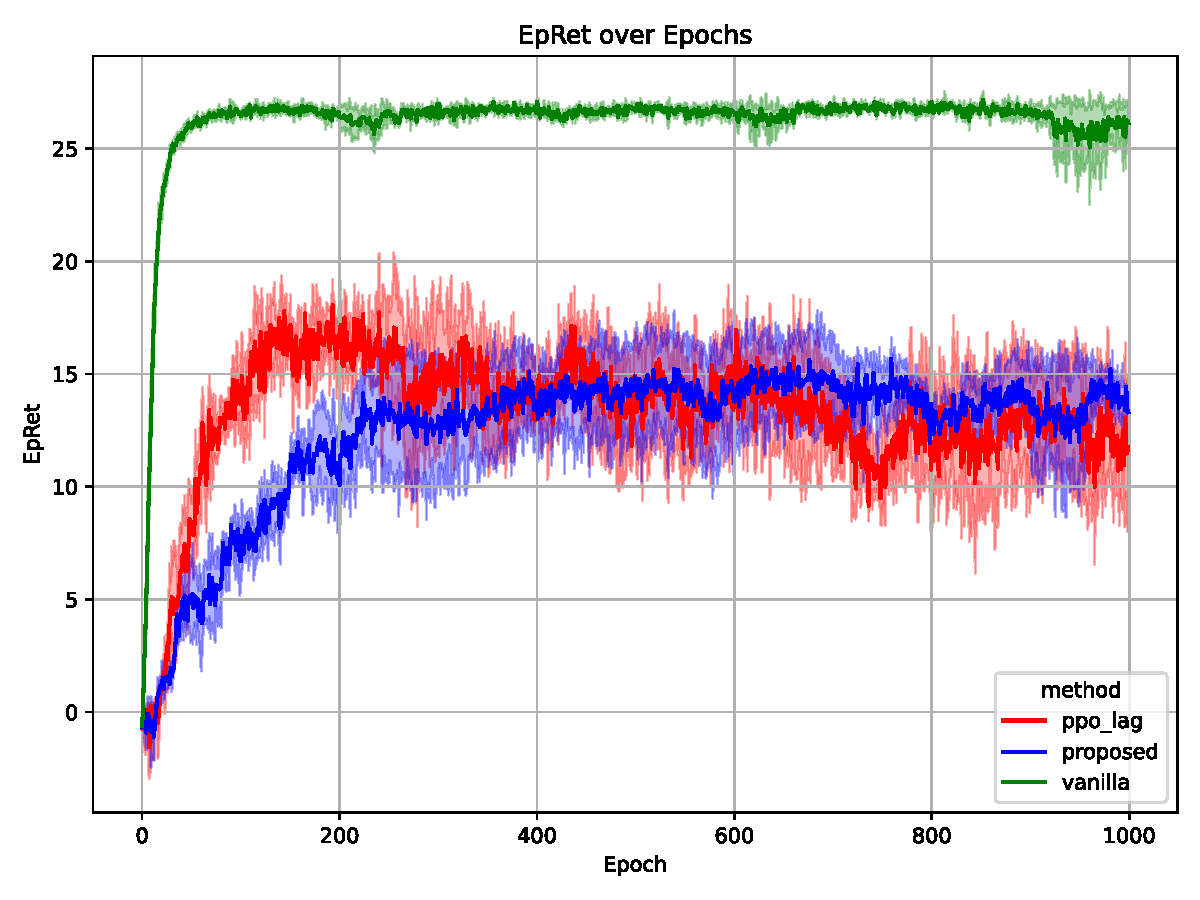
\includegraphics[width=0.45\textwidth]{figures/result_reward.pdf}
      \hspace{1cm}
      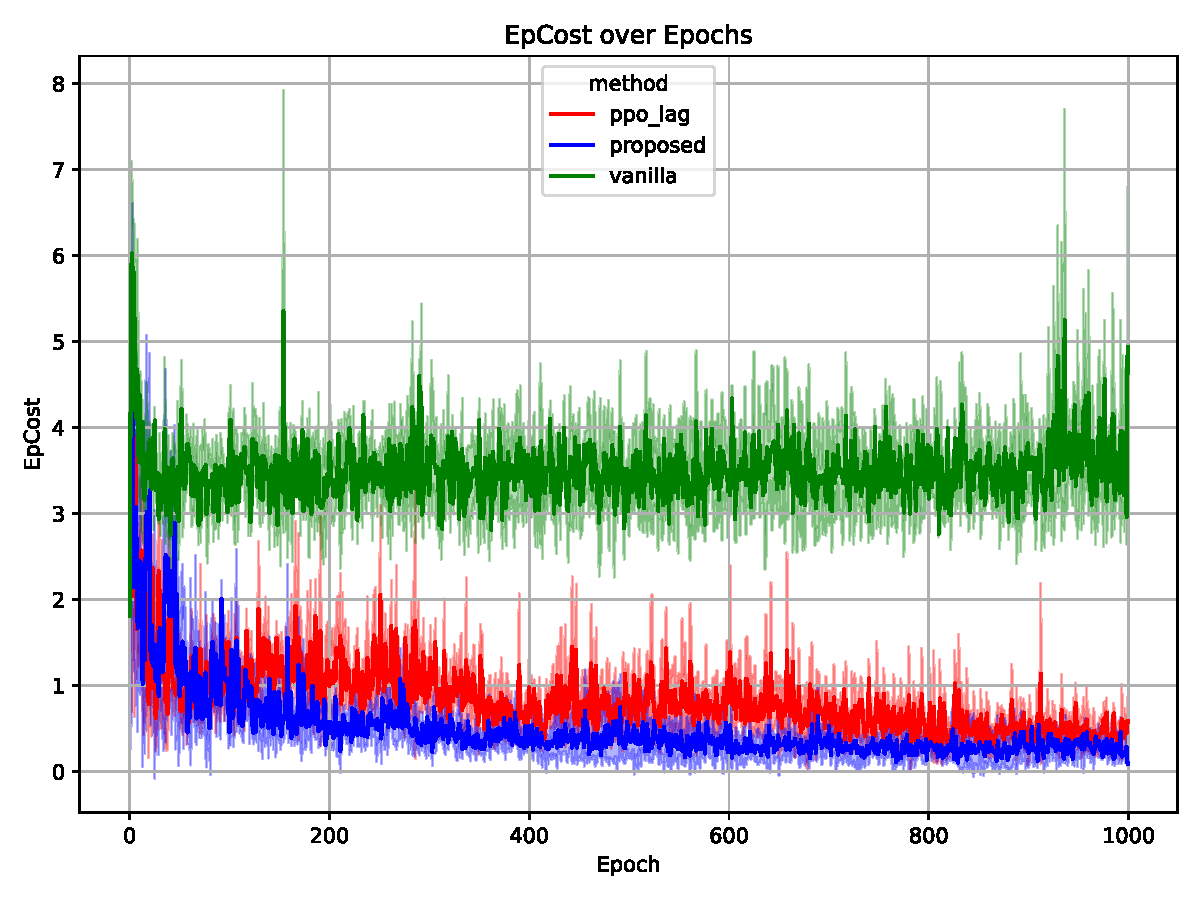
\includegraphics[width=0.45\textwidth]{figures/result_cost.pdf}
      \caption{Performance comparison on Safety Gym tasks}
    \end{figure}
  }

\end{frame}

\begin{frame}{\insertsubsectionhead}{Comparison of Methods}

  \centering
  \begin{columns}[T,totalwidth=\textwidth]
    % PPO
    \column{0.32\textwidth}
      \centering
      \textbf{PPO}
      \includemedia[
        width=\linewidth,
        height=0.5625\linewidth,
        activate=pageopen,
        addresource=figures/ppo-5121.mp4,
        flashvars={source=figures/ppo-5121.mp4&autoPlay=true&loop=true}
      ]{}{VPlayer.swf}

    % PPO Lagrangian
    \column{0.32\textwidth}
      \centering
      \textbf{PPO Lagrangian}
      \includemedia[
        width=\linewidth,
        height=0.5625\linewidth,
        activate=pageopen,
        addresource=figures/ppo_lag-5121.mp4,
        flashvars={source=figures/ppo_lag-5121.mp4&autoPlay=true&loop=true}
      ]{}{VPlayer.swf}

    % Proposed Method
    \column{0.32\textwidth}
      \centering
      \textbf{Proposed Method}
      \includemedia[
        width=\linewidth,
        height=0.5625\linewidth,
        activate=pageopen,
        addresource=figures/ppo_lagnet-5121.mp4,
        flashvars={source=figures/ppo_lagnet-5121.mp4&autoPlay=true&loop=true}
      ]{}{VPlayer.swf}

  \end{columns}

\end{frame}

\begin{frame}{\insertsubsectionhead}{Limitations of the Proposed Method}

  Limitations of the Proposed Approach

  \begin{itemize}
    \item<1-> Sensitivity to Lagrange multiplier (init., learning rate)
    \item<2-> Constraint threshold setting is difficult
      \begin{itemize}
        \item<2-> Too strict → overly conservative policy
        \item<2-> Too lenient → constraints not enforced
      \end{itemize}
    \item<3-> Needs sufficient violations during training
  \end{itemize}

\end{frame}

% ============================================
%         Conclusion Page
% ============================================


\section{Conclusion}

%~~~~~~~~~~~~~~~~~~~~~~~~~~~~~~~~~~~~~~~~~~~~~~~~~~~~~~~~~~~~~~~~~~~~~~~~~~~~~~
\subsection{Summary}

\begin{frame}{\insertsubsectionhead}

  \begin{itemize}
    \item <2-> Major companies focus on supervised learning for autonomous driving
    \item <3-> Supervised learning is costly and data-dependent
    \item <4-> Reinforcement learning can learn policies in simulation and transfer to the real world
    \item <5-> Risk of unsafe behavior due to the Sim2Real gap
    \item <6-> Research direction: state-wise constrained policy learning
  \end{itemize}

  \vspace{0.5cm}

  \uncover<7->{\textbf{But there are still challenges to solve..}}

\end{frame}

%~~~~~~~~~~~~~~~~~~~~~~~~~~~~~~~~~~~~~~~~~~~~~~~~~~~~~~~~~~~~~~~~~~~~~~~~~~~~~~

\subsection{Future Work}

\begin{frame}{\insertsubsectionhead}

  \begin{itemize}
    \item <2-> Extension to Model-Based RL
  \end{itemize}

\end{frame}

%~~~~~~~~~~~~~~~~~~~~~~~~~~~~~~~~~~~~~~~~~~~~~~~~~~~~~~~~~~~~~~~~~~~~~~~~~~~~~~

% ============================================
%         Thank you Page
% ============================================

\section{}
\begin{frame}{}
    \centering \Large
    \emph{Thank you for your attention!}
\end{frame}
%~~~~~~~~~~~~~~~~~~~~~~~~~~~~~~~~~~~~~~~~~~~~~~~~~~~~~~~~~~~~~~~~~~~~~~~~~~~~~~

%~~~~~~~~~~~~~~~~~~~~~~~~~~~~~~~~~~~~~~~~~~~~~~~~~~~~~~~~~~~~~~~~~~~~~~~~~~~~~~
\begin{frame}[allowframebreaks]{References}

  \bibliography{localRefs}
  \bibliographystyle{IEEEtran}

\end{frame}
%~~~~~~~~~~~~~~~~~~~~~~~~~~~~~~~~~~~~~~~~~~~~~~~~~~~~~~~~~~~~~~~~~~~~~~~~~~~~~~

\end{document}